
\begin{minipage}[c]{.4\linewidth}
  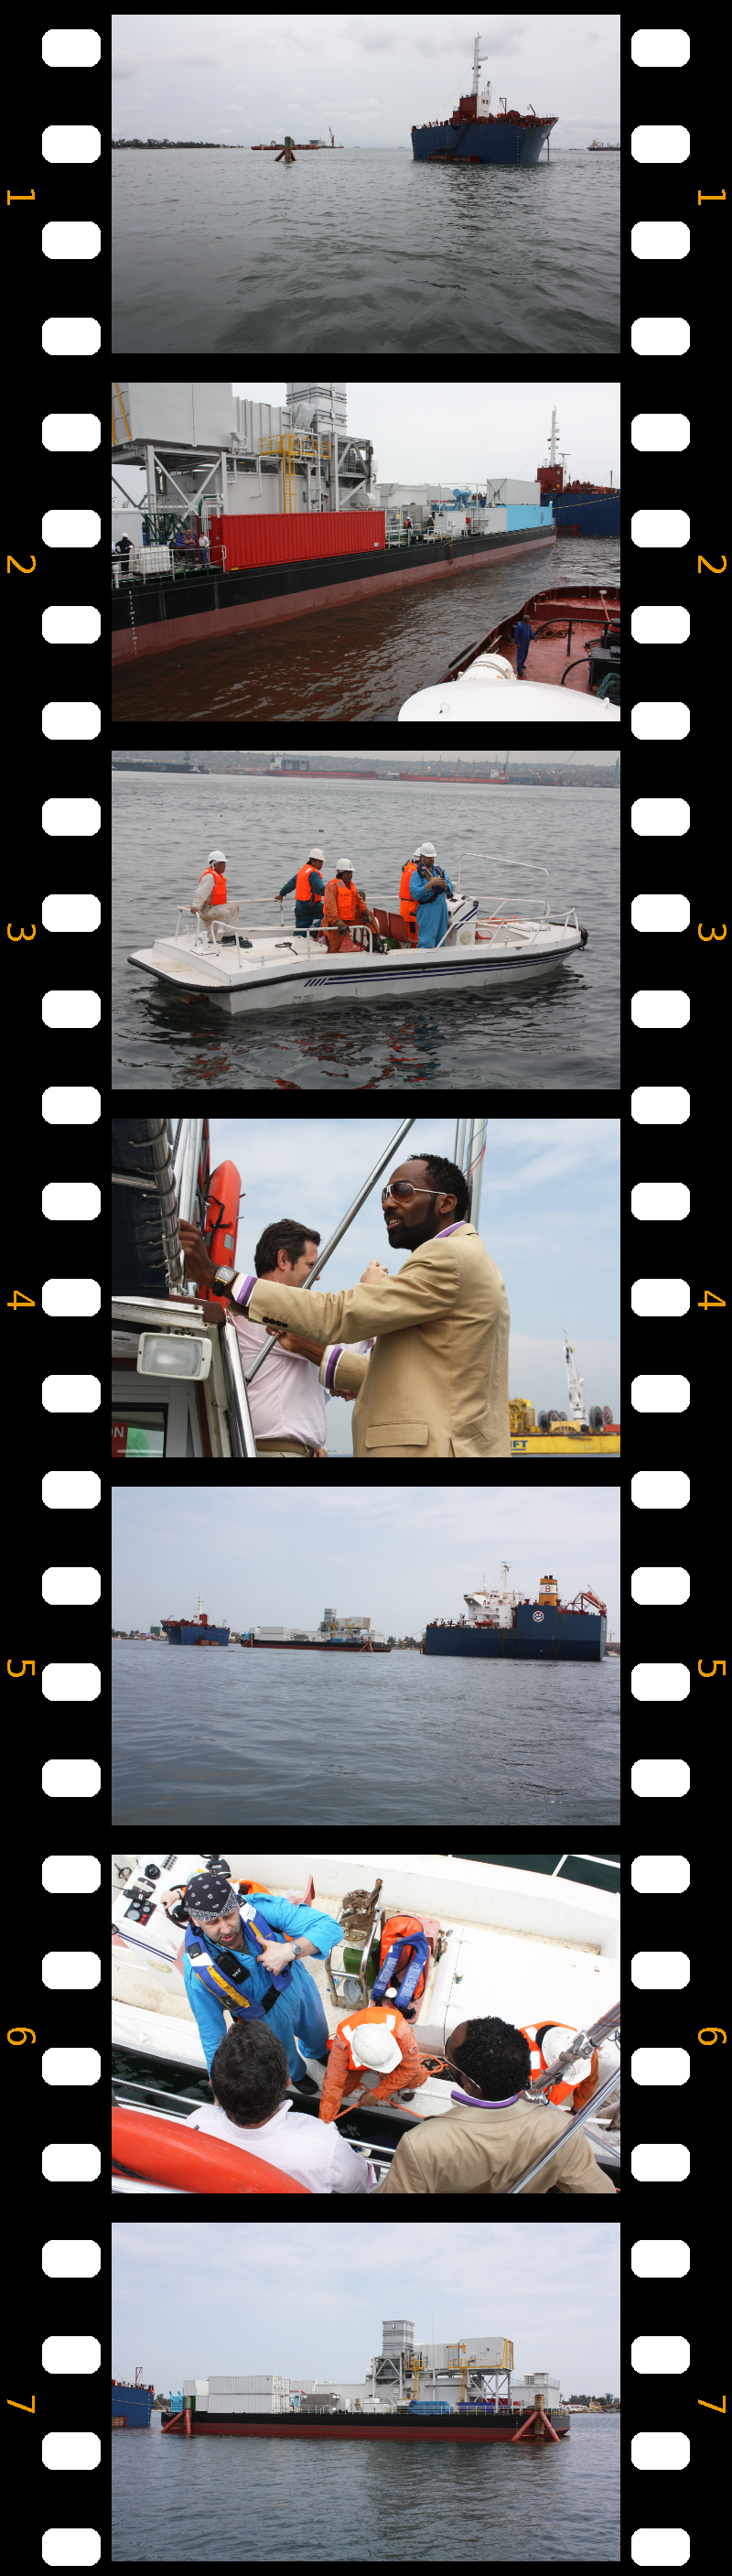
\includegraphics[height=\textheight]{filmVertP1.png}
\end{minipage}\hfill
\begin{minipage}[c]{.55\linewidth}
\cappar The April, 2nd, 2011, the floating power plant Boavista II
parted from Ría de Vigo to Luanda, Angola, on the semisubmergible
vessel Eagle. The boarding manoeuvre and later
transfer to Luanda put an end to a project initiated in October
2009, the first one in Spain for the construction of a floating power
plant. After two weeks of travel, the floating power plant was placed
in its final location inside the dock of Luanda, where the necessary
previous works for the final testing regarding energy load
and supply to the grid will take place.

\vspace{1cm}

The Ministry of Energy and Waters of the Republic of Angola is
enhancing the growth of energy infrastructures and power
production installations as a way to develop the country’s
industry, which will benefit its citizens. One the projects ordered
by the Ministry, represented by Minister Miss Emanuel Vieira
Lopes, has been the project Boavista II, which consists on the
supply of a 42.1 MW gas turbine and its auxiliary equipment
installed in a pontoon. This floating power plant will supply
enough power to cover the needs of 70,000 Angolans.

\vspace{1cm}

As required by a project of these characteristics, project Boavista
II has been developed with the participation of a
multidisciplinary group of companies. The project was awarded
to the consortium comprised by Spanish companies “Comercial
Cueto 92 Internacional” and “Soluciones de Gestión y Apoyo a
Empresas”, with the collaboration of “Idom” for engineering
duties and technical assistance by technicians, “Astilleros P.
Freire” for the construction of the pontoon and the assembling of
the equipment, and suppliers for the most important pieces of
equipment: General Electric for the turbine, ABB for the power
transformer and Alstom Grid (formerly Areva T\&D) for the gasinsulated
substation.

\vspace{1cm}

The engineering, equipment supply, assembling and
commissioning of the systems have been done during 17 months
of work.

\end{minipage}

\newpage

\begin{minipage}[c]{0.9\linewidth}
\vspace{1cm}  

\section{General description of the installation}
The installation consists on a pontoon over which a turbogenerator
group has been installed. Its generated electric
energy is evacuated to the ground by a high voltage power line.



The electric generator group is comprised by the following
equipments: GE 6B turbine, mounting systems, electric
generator, main transformer and GIS substation. All these main
equipments are placed over the pontoon. The plan also has the
following auxiliary systems and services: emergency
generators sets, fireproofing systems, water treatment plant,
compressed air plant, control rooms, pumping room, power
system room, gasoil tanks, water tanks and storage rooms.



The electric connection for the exportation of energy with the
dock takes place trough an isolated cable supported by an
output porch and the supply of process and service fluids
trough flexible pipes.

\vspace{1cm}  

\section{Loading and unload manoeuvre}

The loading manoeuvre of this 1,206 m2, 1,700 t. pontoon
started with two tug boats that worked for 35 minutes to tug
the pontoon from the reparation dock in Bouzas. An hour was
needed to put it in position over the deck of the special tug
boat Eagle, submerged 5.5 m. under the sea since several hours
before. Once the pontoon was set, the ship emerged from water
with the pontoon over its cover, completing the loading
operation for which a total of 6 hours were required.

14 days later, and after travelling for the 6,500 km. that
separate the coasts of Vigo and Luanda, the ship by the
company Offshore Heavy Transport, one of the few companies
with submergible ships, submerged again to free the pontoon
in its destination. It was decided that this transport modality
was the best after studying other possibility, wchich would
have been tugging the pontoon through the ocean, with all the
risks it would have involved during the loading process.\\

\vspace{1cm}  

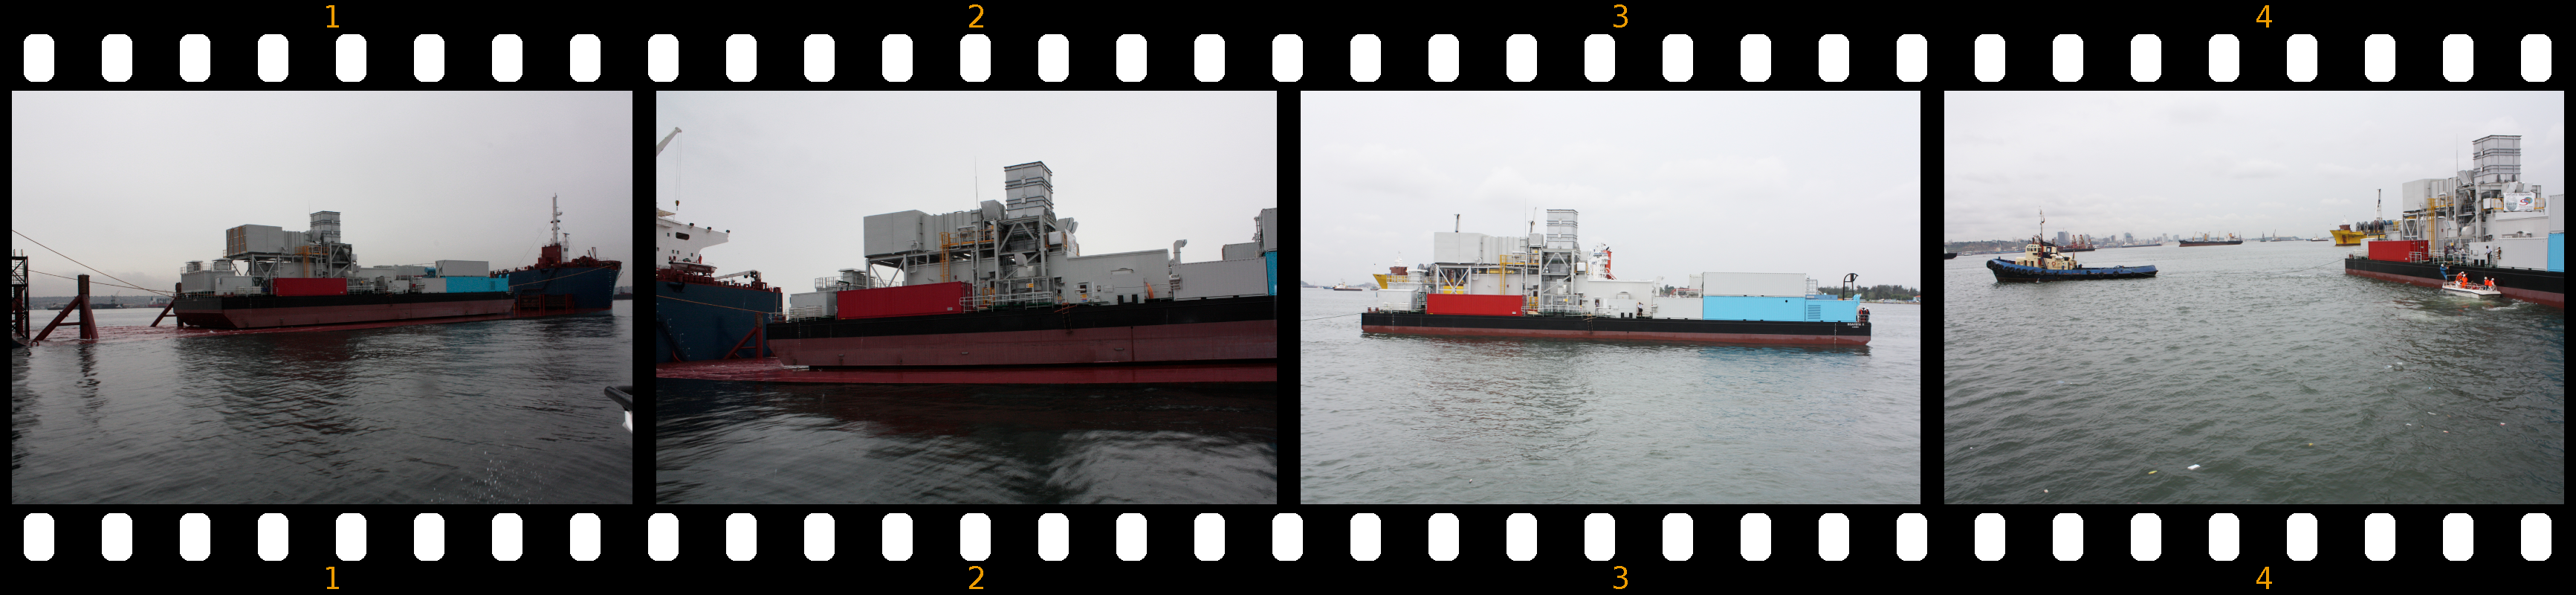
\includegraphics[width=\textwidth]{filmHorP2.png}


\end{minipage}
\newpage
%%% Local Variables: 
%%% mode: latex
%%% TeX-master: "novedades"
%%% End: 


